\documentclass[12pt]{article}

% === Packages ===
\usepackage[english]{babel}
\usepackage{amsmath, amssymb}
\usepackage{graphicx}
\usepackage{float}
\usepackage{subcaption}
\usepackage{tikz, pgfplots}
\usetikzlibrary{positioning}
\usepackage{geometry}
\usepackage{fancyhdr}
\usepackage{hyperref}
\usepackage{xcolor}
\usepackage{titlesec}
\usepackage{enumitem}
\usepackage{url}

% === Geometry ===
\geometry{
  a4paper,
  total={170mm,257mm},
  left=25mm,
  right=25mm,
  top=30mm,
  bottom=30mm,
}

% === Header ===
\pagestyle{fancy}
\fancyhf{}
\lhead{Obstacle-Aware UAV Guidance}
\rhead{Heavenly Dadala}
\cfoot{\thepage}

% === Title Page Macro ===
\newcommand{\maketitlepage}{
\begin{titlepage}
    \centering
    \vspace*{2.5cm}

    {\Huge \bfseries Obstacle-Aware Waypoint Tracking for UAVs}\\[0.4cm]
    {\Large Using SCS Switching and L1 Nonlinear Guidance}\\[1.8cm]

    \begin{flushleft}
    \textbf{Author:} \\[0.2cm]
    Heavenly Dadala \\
    Undergraduate Researcher \\
    Department of Aerospace Engineering \\
    Indian Institute of Technology Kharagpur
    \end{flushleft}

    \vspace{1.3cm}

    \begin{flushleft}
    \textbf{Supervisor:} \\[0.2cm]
    Prof. Shikha Hota \\
    Department of Aerospace Engineering \\
    Indian Institute of Technology Kharagpur
    \end{flushleft}

    \vfill

    \begin{flushleft}
    \textbf{Version:} 1.1 \\
    \textbf{Last Updated:} July 3, 2025 \\
    \textbf{GitHub:} \url{https://github.com/Heavenly-cyber/Obstacle_avoidance_waypoints}
    \end{flushleft}

    \vspace{1.2cm}
    \begin{center}
    \large \today
    \end{center}
\end{titlepage}
}

% === Document Starts ===
\begin{document}

\pagenumbering{gobble}
\maketitlepage

\tableofcontents
\newpage

\pagenumbering{arabic}

\section{Introduction}
In UAV trajectory tracking, obstacles like restricted zones can appear between waypoints. The goal is to smoothly guide the UAV around these zones without violating safety buffers or sacrificing tracking accuracy.

\section{Proposed Guidance Method}
We adopt a three-phase Straight-Circle-Straight (SCS) strategy integrated with L1 guidance. The UAV dynamically computes entry and exit points for the obstacle-avoidance maneuver using tangents to the obstacle's circular danger zone. These transitions are smoothened with blending and enforced with distance and direction locks.

\subsection{Straight-Line Convergence}
We use vector projection to compute the reference point on the line segment and generate lateral acceleration using L1 logic:
\begin{itemize}
  \item Project UAV's position onto line.
  \item Compute L1 vector from UAV to reference point.
  \item Generate lateral acceleration based on angular deviation $\eta$.
\end{itemize}

\subsection{Circular Convergence}
For avoiding circular obstacles, L1 guidance tracks a circular arc:
\begin{itemize}
  \item Compute angle from UAV to circle center.
  \item Compute entry/exit using tangent points.
  \item Track arc with adjusted heading until exit point.
\end{itemize}

\subsection{Mode Switching}
We use a 3-mode SCS system:
\begin{itemize}
  \item Mode 1: Straight Line to Entry Point
  \item Mode 2: Arc Tracking from Entry to Exit
  \item Mode 3: Straight Line to Next Waypoint
\end{itemize}
Each mode transition is triggered by reaching its respective target within a threshold.

\section{Implementation Details}
\begin{itemize}
  \item Language: MATLAB
  \item Simulation: Discrete 2D simulator
  \item L1 Distance: Tuned per mode and test
  \item Smoothing: Blending functions over 5–10 seconds
  \item Transition Detection: Euclidean distance to reference points
  \item Plots: Curvature, mode switch timeline, lateral acceleration
\end{itemize}

\section{Results}
\begin{itemize}
  \item Path tracking was successful across 10 waypoints.
  \item The UAV strictly avoided the obstacle buffer.
  \item Curvature and lateral acceleration stayed within safe bounds.
\end{itemize}

\begin{figure}[H]
  \centering
  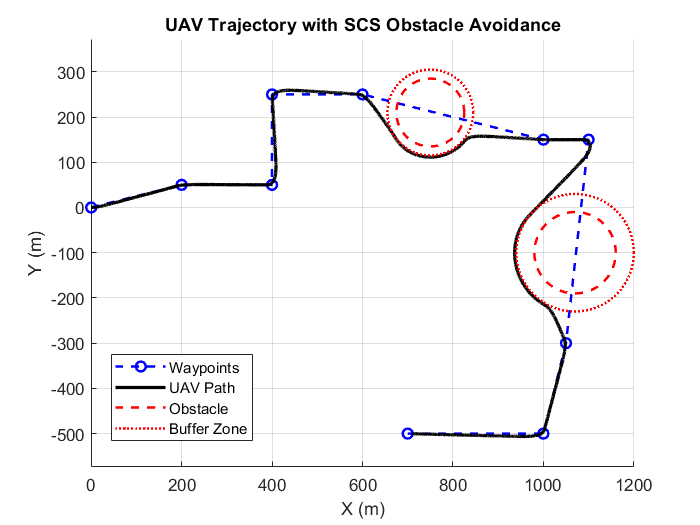
\includegraphics[width=0.8\textwidth]{images/Final_work1.png}
  \caption{Final UAV Trajectory with Obstacle Avoidance}
\end{figure}

\begin{figure}[H]
  \centering
  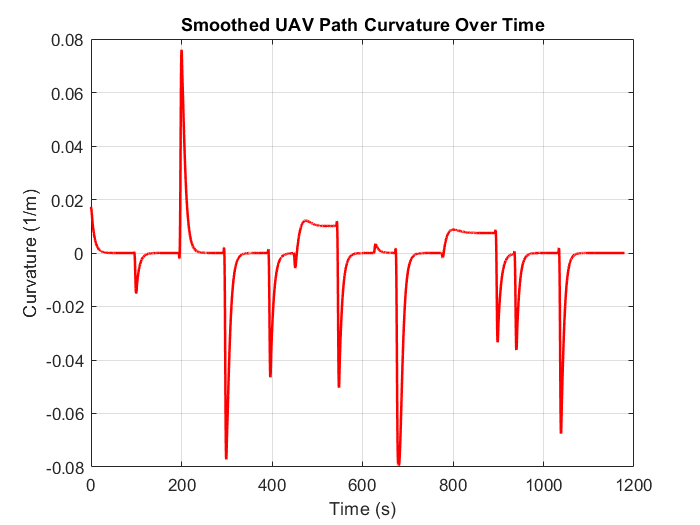
\includegraphics[width=0.8\textwidth]{images/Curvature_after_smooth.png}
  \caption{Path Curvature After Smoothing}
\end{figure}

\begin{figure}[H]
  \centering
  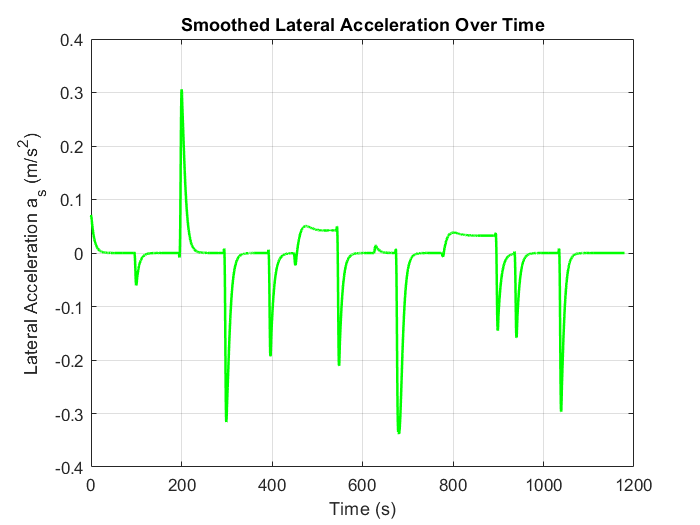
\includegraphics[width=0.8\textwidth]{images/Lateral_acc.png}
  \caption{Lateral Acceleration Over Time}
\end{figure}

\section{Conclusion}
The proposed L1-based SCS strategy with tangent-based transitions and smoothing effectively solves the problem of obstacle-aware waypoint tracking. The system maintains safety, robustness, and trajectory fidelity. This foundation can be extended to dynamic and 3D path planning.

\section*{References}
\begin{enumerate}[label={[\arabic*]}]
  \item S. Park et al., "A New Nonlinear Guidance Logic for Trajectory Tracking," MIT, 2004.
  \item J. Saunders, R. W. Beard, and T. McLain, "Obstacle Avoidance Using Circular Paths," AIAA Guidance, Navigation, and Control Conference, 2007.
  \item Y. Yaniv, I. Shmuel, and T. Shima, "Path Following Based on Waypoints and Real-Time Obstacle Avoidance," Aerospace Science and Technology, 2022.
\end{enumerate}

\end{document}
